\documentclass[border=3pt]{standalone}
% Preâmbulo compartilhado pelos diagramas TikZ da aula 9 de IHC (Princípios e Diretrizes)
\usepackage[T1]{fontenc}
\usepackage[utf8]{inputenc}
\usepackage{lmodern}
\usepackage{amsmath}
\usepackage{xcolor}
\usepackage{tikz}
\usetikzlibrary{arrows.meta,angles,quotes,decorations.pathmorphing,decorations.pathreplacing,calc,
                positioning,shapes.geometric,shapes.misc,backgrounds,fit,
                math}

% Paleta (mesma dos SVGs originais)
% Paleta da disciplina de IHC: acento roxo (#755099), da capa do livro.
% (o nome "dblue" é mantido para não alterar todos os diagramas)
\definecolor{dblue}{HTML}{755099}
\definecolor{dorange}{HTML}{B3541E}
\definecolor{dgreen}{HTML}{4A7C59}
\definecolor{dred}{HTML}{9C4B4B}
\definecolor{dcream}{HTML}{F4F1EA}
\definecolor{dshade}{HTML}{DDD7C9}

% Função gaussiana (não normalizada por padrão de escala visual)
\pgfmathdeclarefunction{gauss}{3}{%
  \pgfmathparse{1/(#3*sqrt(2*pi))*exp(-((#1-#2)^2)/(2*#3^2))}%
}

% Estilos comuns (prefixo d... para não colidir com chaves internas do pgf)
\tikzset{
  >={Stealth[length=2mm]},
  dguide/.style={gray!55, dashed, line width=0.4pt},
  daxis/.style={gray!60, line width=0.7pt, ->},
  dbody/.style={fill=black!3, draw=black!80, line width=1pt},
  dacc/.style={draw=dblue, line width=1pt},
  dlbl/.style={black!55, font=\small},
  dsub/.style={black!45, font=\footnotesize},
  dstate/.style={circle, draw=black!80, fill=dcream, line width=1pt,
                 minimum size=17mm, font=\large, inner sep=1pt},
  dobs/.style={circle, draw=black!80, fill=dshade, line width=1pt,
               minimum size=14mm, font=\large, inner sep=1pt},
  dbox/.style={rounded corners=2pt, draw=black!80, fill=dcream, line width=1pt,
               align=center, inner sep=6pt},
  dop/.style={circle, draw=black!80, fill=white, line width=1pt,
              minimum size=6mm, inner sep=0pt, font=\small},
  dtrans/.style={->, dblue, line width=1pt},
  dmeas/.style={->, dorange, line width=1pt},
  dcurve/.style={line width=1pt, dblue},
  dcurveb/.style={line width=1.4pt, dorange},
}

\begin{document}
\hyphenpenalty=10000 \exhyphenpenalty=10000 \tolerance=9999 \emergencystretch=3em
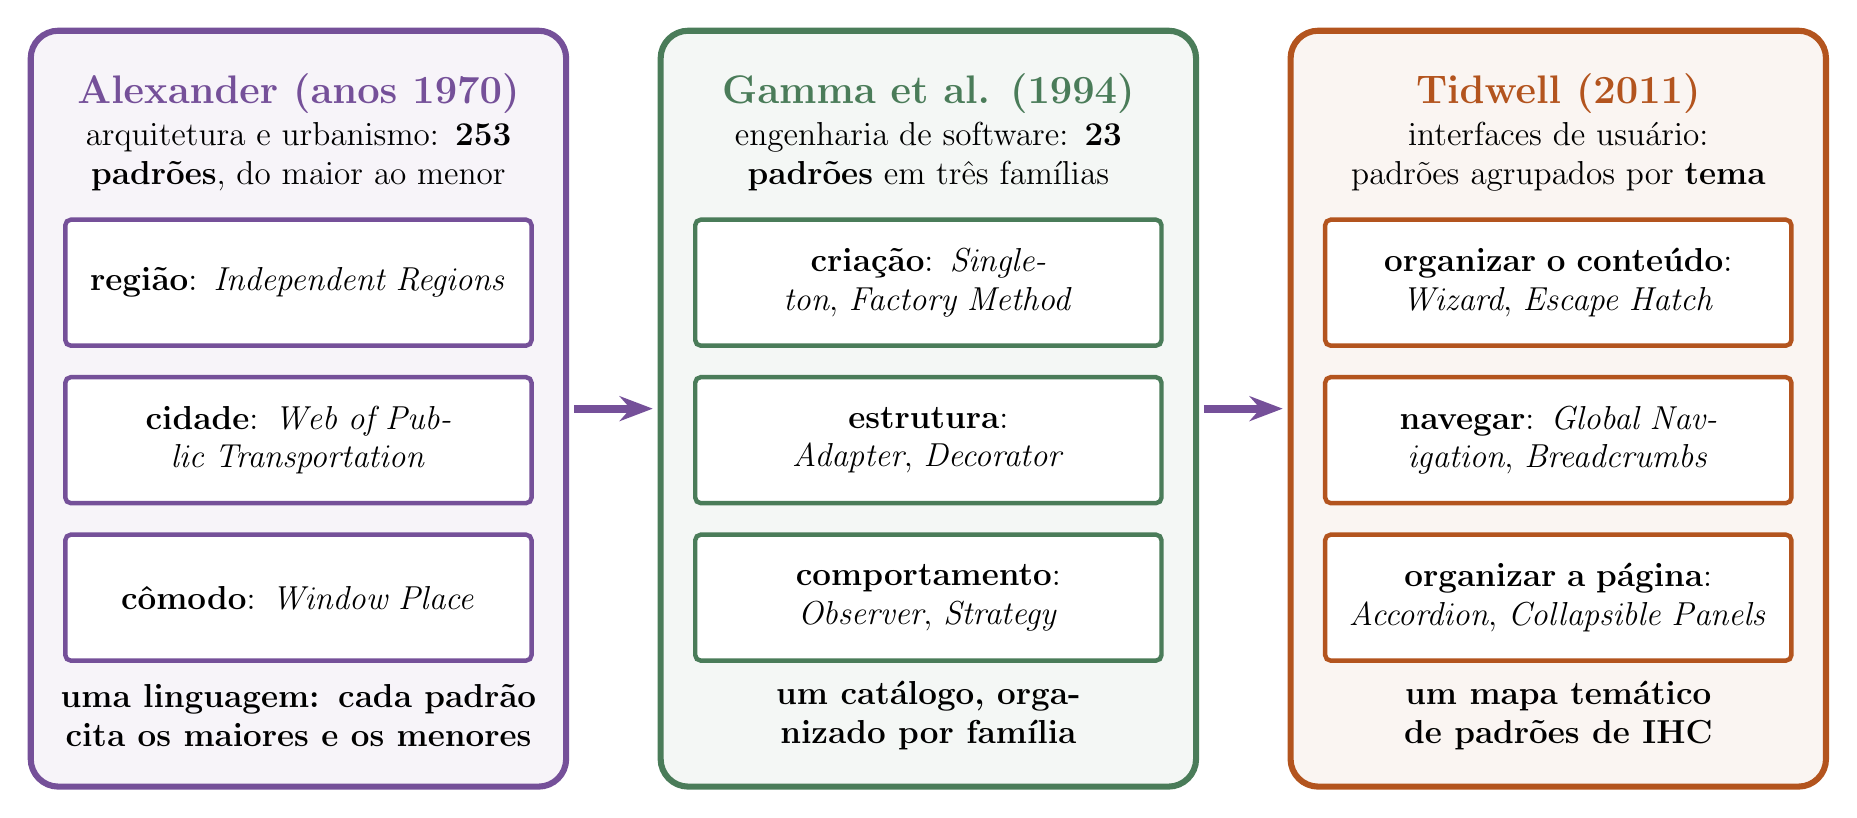
\begin{tikzpicture}[x=1cm,y=1cm]
\draw[draw=dblue, line width=2.2pt, fill=dblue!6, rounded corners=10pt] (0.0,-0.4) rectangle (6.8,9.2);
\node[font=\Large\bfseries, text=dblue] at (3.4,8.4) {Alexander (anos 1970)};
\node[font=\large, text width=6.2cm, align=center] at (3.4,7.6) {arquitetura e urbanismo: \textbf{253 padrões}, do maior ao menor};
\node[dbox, draw=dblue, text width=5.5cm, minimum height=1.6cm, font=\large, line width=1.6pt, fill=white] (blue6) at (3.4,6.0) {\textbf{região}: \emph{Independent Regions}};
\node[dbox, draw=dblue, text width=5.5cm, minimum height=1.6cm, font=\large, line width=1.6pt, fill=white] (blue4) at (3.4,4.0) {\textbf{cidade}: \emph{Web of Public Transportation}};
\node[dbox, draw=dblue, text width=5.5cm, minimum height=1.6cm, font=\large, line width=1.6pt, fill=white] (blue2) at (3.4,2.0) {\textbf{cômodo}: \emph{Window Place}};
\node[font=\large\bfseries, text width=6.2cm, align=center] at (3.4,0.5) {uma \textbf{linguagem}: cada padrão cita os maiores e os menores};
\draw[draw=dgreen, line width=2.2pt, fill=dgreen!6, rounded corners=10pt] (8.0,-0.4) rectangle (14.8,9.2);
\node[font=\Large\bfseries, text=dgreen] at (11.4,8.4) {Gamma et al. (1994)};
\node[font=\large, text width=6.2cm, align=center] at (11.4,7.6) {engenharia de software: \textbf{23 padrões} em três famílias};
\node[dbox, draw=dgreen, text width=5.5cm, minimum height=1.6cm, font=\large, line width=1.6pt, fill=white] (green6) at (11.4,6.0) {\textbf{criação}: \emph{Singleton}, \emph{Factory Method}};
\node[dbox, draw=dgreen, text width=5.5cm, minimum height=1.6cm, font=\large, line width=1.6pt, fill=white] (green4) at (11.4,4.0) {\textbf{estrutura}: \emph{Adapter}, \emph{Decorator}};
\node[dbox, draw=dgreen, text width=5.5cm, minimum height=1.6cm, font=\large, line width=1.6pt, fill=white] (green2) at (11.4,2.0) {\textbf{comportamento}: \emph{Observer}, \emph{Strategy}};
\node[font=\large\bfseries, text width=6.2cm, align=center] at (11.4,0.5) {um \textbf{catálogo}, organizado por família};
\draw[draw=dorange, line width=2.2pt, fill=dorange!6, rounded corners=10pt] (15.999999999999998,-0.4) rectangle (22.799999999999997,9.2);
\node[font=\Large\bfseries, text=dorange] at (19.4,8.4) {Tidwell (2011)};
\node[font=\large, text width=6.2cm, align=center] at (19.4,7.6) {interfaces de usuário: padrões agrupados por \textbf{tema}};
\node[dbox, draw=dorange, text width=5.5cm, minimum height=1.6cm, font=\large, line width=1.6pt, fill=white] (orange6) at (19.4,6.0) {\textbf{organizar o conteúdo}: \emph{Wizard}, \emph{Escape Hatch}};
\node[dbox, draw=dorange, text width=5.5cm, minimum height=1.6cm, font=\large, line width=1.6pt, fill=white] (orange4) at (19.4,4.0) {\textbf{navegar}: \emph{Global Navigation}, \emph{Breadcrumbs}};
\node[dbox, draw=dorange, text width=5.5cm, minimum height=1.6cm, font=\large, line width=1.6pt, fill=white] (orange2) at (19.4,2.0) {\textbf{organizar a página}: \emph{Accordion}, \emph{Collapsible Panels}};
\node[font=\large\bfseries, text width=6.2cm, align=center] at (19.4,0.5) {um \textbf{mapa temático} de padrões de IHC};
\draw[dtrans, line width=3pt, -{Stealth[length=4.2mm]}] (6.9,4.4) -- (7.9,4.4);
\draw[dtrans, line width=3pt, -{Stealth[length=4.2mm]}] (14.9,4.4) -- (15.9,4.4);
\end{tikzpicture}
\end{document}
